\chapter{Problématiques de mise en production}


\subsection{Une \gls{chaîne} à mettre en place}

Le choix d'un algorithme ou d'un modèle pour accomplir une tâche donnée n'est que la première étape vers le développement d'une solution d'automatisation basée sur du \emph{machine learning}. 
Le modèle sélectionné traite des données en entrée et génère une sortie, qui doit ensuite être intégrée dans une \gls{chaîne} plus large. 
Ces données de sortie ne sont en effet pas directement exploitables en l'état. 
Dans cette section, nous décrivons la chaîne de traitement mise en place pour le projet InventAIre, afin de prendre du recul, en analysant ses forces et ses faiblesses.

Le schéma ci-dessous résume ce processus général de traitement mis en place, qui sera expliqué plus en détail, étape par étape.\newline
\begin{figure}[h!]
	\centerline{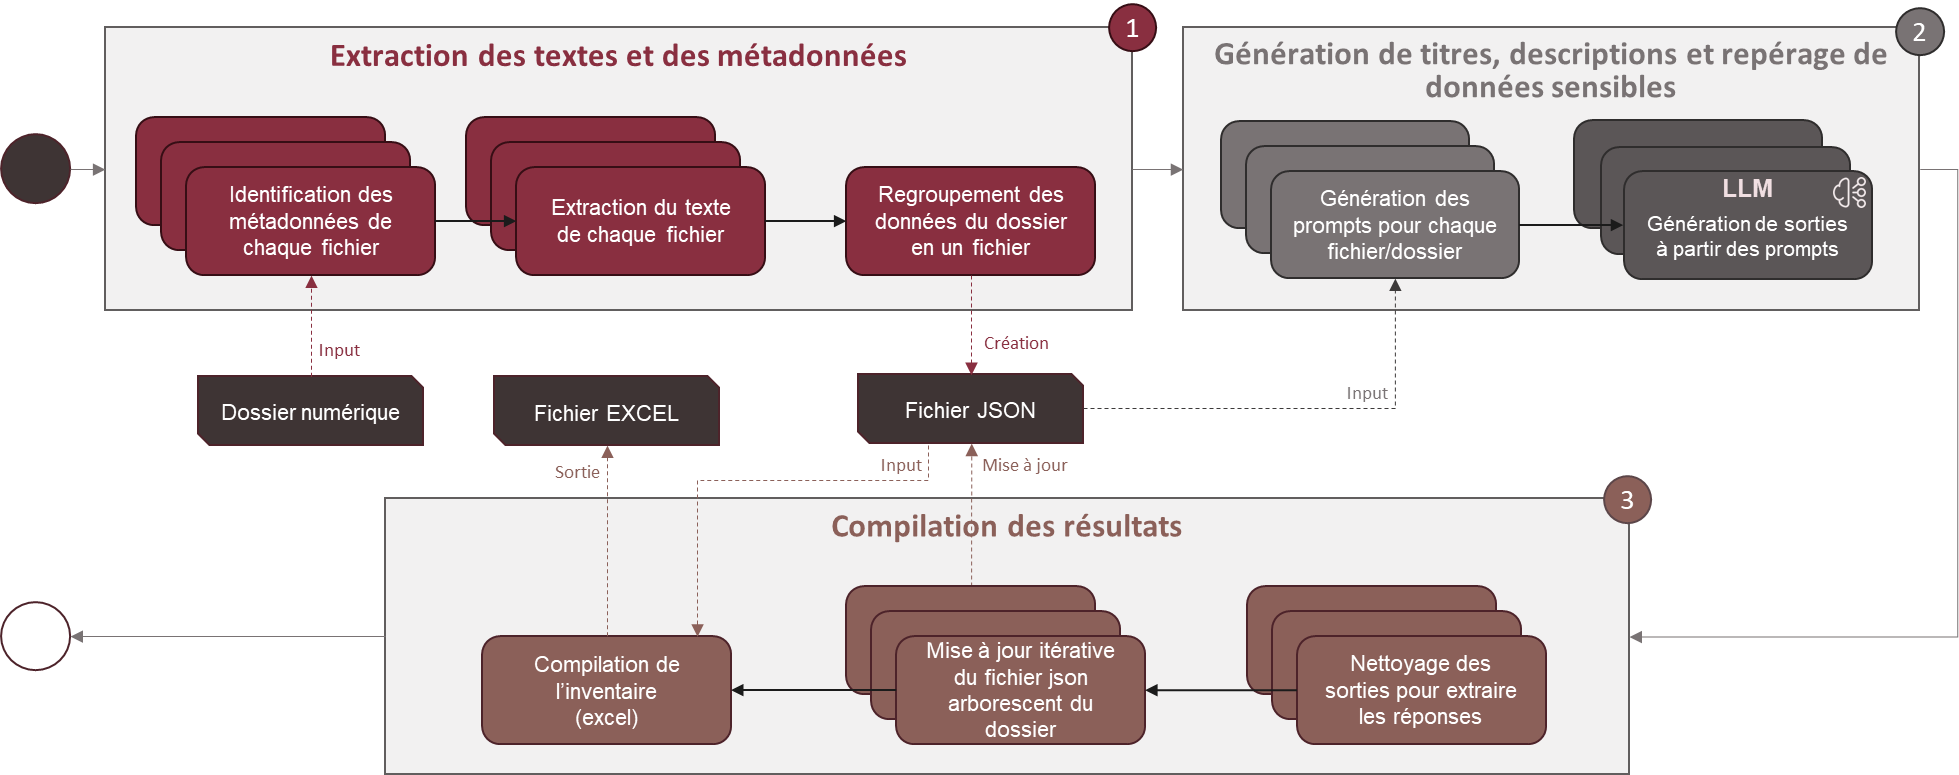
\includegraphics[width=\textwidth]{./media/process_traitement.png}}
	\caption{Processus de traitement mis en place afin de générer l'inventaire}
\end{figure}

\paragraph*{Étape 1 : Extraction des textes et des métadonnées des documents}\mbox{}\\

L'application prend en entrée un chemin de répertoire numérique.
Les métadonnées extractibles de l'intégralité du contenu de ce dernier sont compilées en un seul un fichier au format JSON, 
avec le texte de chaque document. Si le texte n'est pas disponible, une tentative d'océrisation est réalisée avec le logiciel Tesseract.
Dans le cas où les textes des fichiers seraient trop grands et dépasseraient la \gls{fenêtre} de Llama 3, ils sont divisés en différentes parties,
 que nous avons nommées \enquote{chunks}, de 10 000 caractères. Ce découpage est relativement arbitraire, nous aurions pu couper 
 au niveau de la fin d'une phrase pour que cela perturbe moins notre LLM.
 Nous aurions également pu tester avec des chevauchements entre les différents \enquote{chunks}.
 Ci-dessous se trouve un exemple de fichier JSON arborescent produit pour un dossier qui contiendrait un seul document.
 \vspace*{0.2cm}
\begin{tcolorbox}[colback=white, colbacktitle=white, coltitle=black, title=Exemple de fichier JSON arborescent pour un dossier contenant un document, center title]
  \begin{minted}[]{json}
 {
    "path": "C:\User\Chemin\du\dossier_exemple",
    "folderName": "dossier_exemple",
    "type": "directory",
    "content": [
    {
        "path": "C:\User\Chemin\du\dossier_exemple\document.txt",
        "type": "file",
        "fileName": "document.txt",
        "creationDate": "Wed May 20 10:26:26 2024",
        "modificationDate": "Wed May 29 10:35:06 2024",
        "mimeType": "text/plain; charset=UTF-16LE",
        "texte": "Ceci est le texte d'un document txt.",
        "generatedTitle": "to be defined"
    }
    ],
    "generatedTitle": "to be defined"
 }
\end{minted}
\end{tcolorbox}



\paragraph*{Étape 2 : Génération de titres, descriptions et repérage de données sensibles}\mbox{}\\

A partir du document JSON, des \gls{prompt}s sont ensuite générés pour chaque niveau dans l'arborescence et chaque donnée sensible.
Le LLM est interrogé avec ces différents prompts.
L'encadré ci-dessous en montre un exemple.
En rose se trouvent les éléments mutables selon le type d'entrée (document, dossier, chunk) 
et en vert se trouvent les éléments mutables selon la colonne à remplir.

 
\begin{tcolorbox}[colback=white, colbacktitle=white, coltitle=black, title=Exemple de prompt]

\underline{Input :}
\begin{minted}[]{json}
    {
        "path": "C:\User\Chemin\du\dossier_exemple\document.txt",
        "type": "file",
        "fileName": "document.txt",
        "creationDate": "Wed May 20 10:26:26 2024",
        "modificationDate": "Wed May 29 10:35:06 2024",
        "mimeType": "text/plain; charset=UTF-16LE",
        "texte": "Ceci est le texte d'un document txt.",
        "generatedTitle": "to be defined"
    }
\end{minted}

\underline{Context :}
You are an achivist at the Chambre des Députés of Luxembourg.

\underline{Question :}
You have been given a \textcolor{purple}{full document and some metadata} formatted as json as input. You are working on an archival inventory project.
Please generate one \textcolor{teal}{title} \textcolor{teal}{(max 20 words)} in french for this \textcolor{purple}{document} for the inventory.

\textcolor{teal}{In your title, avoid the word 'fonds'. Avoid generic words such as 'divers' or 'variés'. Also avoid the word 'documents' without further precisions : add the types or names of the documents being exhaustive (all of the major types). It would be better if you could format it this way : 'subject, topic - action/type of document', only do it if there is a clear topic or subject and a clear action or only one clear types/names of documents. If there is a chronological indication in your title (not madatory, only if you are sure and if it is pertinent, must be with the topic if it is the date of the event that constitutes the topic) the format is day (number) month (letters, no abbreviation) year (number). If there are several parts in your title, separate them with commas. Be precise and exhaustive in your title (remember : topic/subject - action(s)/precise type(s) of documents if you can) but do not put information you are not sure about. If the document's text does not give you information, do not make it up. Make sure to mention the important people, organizations, locations, dates, ... if you identify some.}

Examine well the whole content for this. Please only write the \textcolor{teal}{title} in french, nothing else, so I can directly reuse it in my inventory. 
Do not explain your answer or tell me about alternatives in your answer. I only need the \textcolor{teal}{title}. Do not invent information, only use the ones you have. 
It's ok if your answer is minimalist because you do not have enough info.
\textcolor{purple}{Be careful, sometimes a file contains several types of document.}

Make sure the syntax and spelling in french in your answer are correct.

\textcolor{teal}{title} in french :


\end{tcolorbox}

Quand le document est un dossier, c'est une arborescence plus grande qui est donnée en entrée, avec des titres et descriptions déjà générés, parce que l'ensemble des textes serait trop long et dépasserait la fenêtre du \emph{LLM}. Il en va de même pour la génération d'un titre ou d'une description pour un document composé de \enquote{chunks} : un résumé de chaque partie du document est généré
et c'est à partir de ces résumés que sont générés les descriptions et titres de ce dernier.

\paragraph*{Étape 3 : Compilation des résultats obtenus par le \emph{LLM}}\mbox{}\\

Les réponses sont extraites des résultats fournis par le \emph{LLM}~: selon le prompt, on extrait le \enquote{oui}/\enquote{yes}, le \enquote{non}/\enquote{no} ou un pourcentage de probabilité généré
 pour remplir les colonnes sur les données sensibles avec des \enquote{oui} ou des \enquote{non}.
Le fichier JSON est par la suite mis à jour de manière itérative après chaque \gls{inference} du modèle, qui correspond à un prompt.
La mise à jour du fichier JSON part du bas de l'arborescence pour remonter vers la racine. Cela permet de décrire chaque niveau en fonction de son contenu. S'il y a un grand nombre de niveaux,
 les niveaux supérieurs seront décrits en fonction du titre et de la description générés pour les dossiers et fichiers qu'ils contiennent.
 L'avantage est la description de chaque niveau. Les données sensibles repérées sont également compilées au fur et à mesure par niveau.
 Un inconvénient réside dans le fait que la description est de moins en moins précise en remontant dans l'arborescence. Les erreurs sur les données sensibles s'ajoutent également, 
 le niveau supérieur d'une grosse arborescence contient donc en général beaucoup de données sensibles alors que ce n'est pas forcément le cas.
 
 Une fois l'inférence réalisée sur l'ensemble du fichier JSON et pour toutes les colonnes de l'inventaire,
 ce dernier est compilé en un fichier Excel avec une ligne par niveau dans l'arborescence.\newline
 
 
 \begin{figure}[h!]
 	\centerline{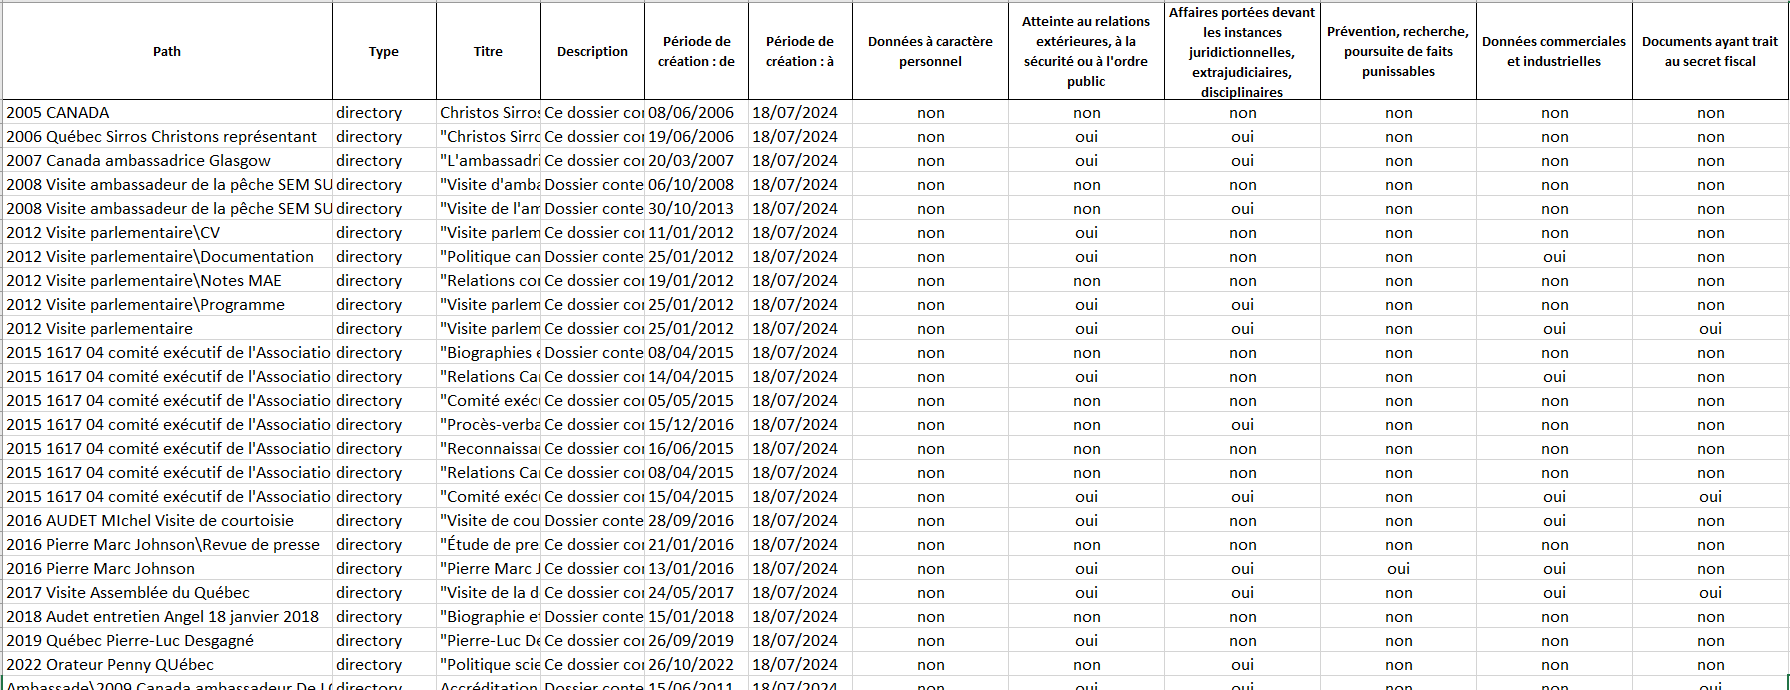
\includegraphics[width=12cm]{./media/results.png}}
 	\caption{Exemple de tableau Excel contenant les résultats d'une inférence}
 \end{figure}
 
 
\begin{figure}[h!]
	\centerline{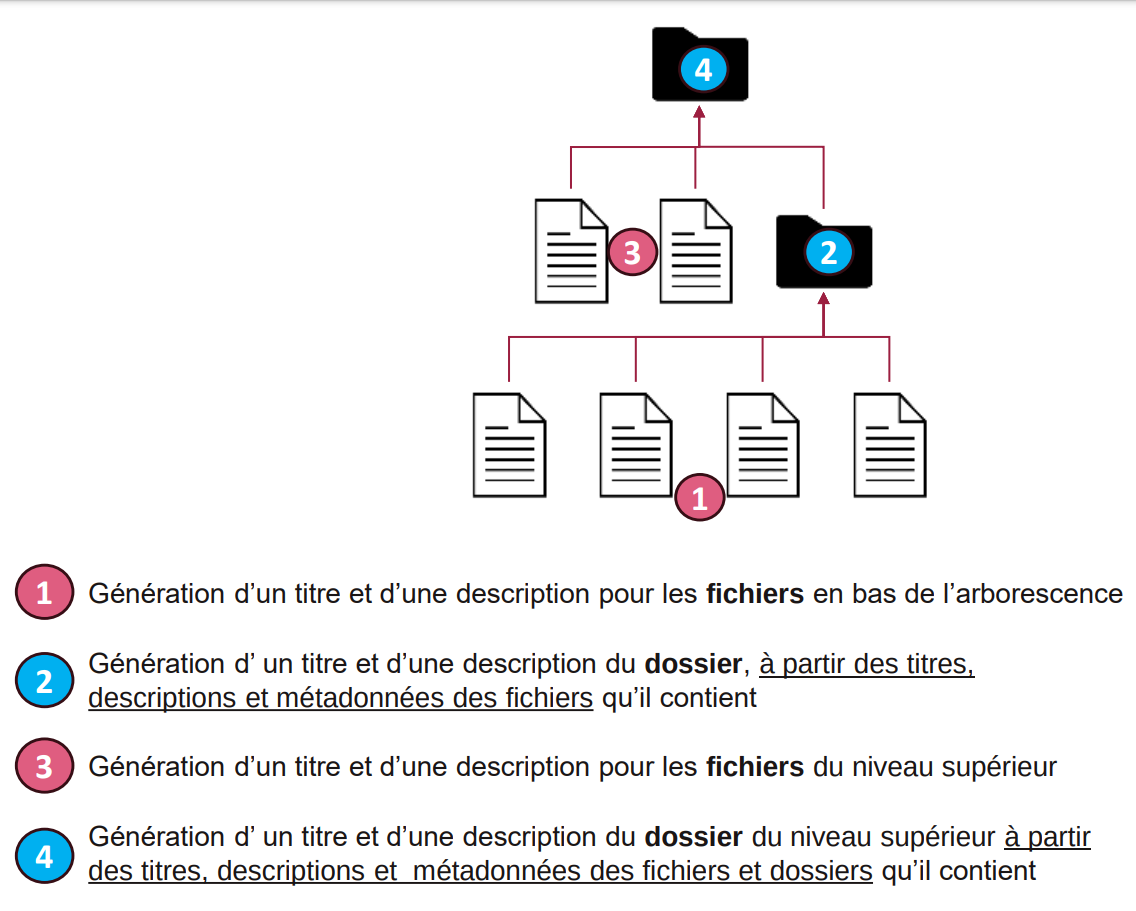
\includegraphics[width=12cm]{./media/remplissage_json.png}}
	\caption{Schéma du fonctionnement de l'inférence pour traiter chaque niveau d'arborescence dans le cas de la génération de titres et descriptions}
\end{figure}





Avec un peu de recul, nous pouvons dire que cette chaîne de traitement et le code en général sont assez complexes. Elle n'est pas composé de beaucoup d'étapes très distinctes les unes des autres, 
mais le traitement itératif pour chaque niveau de l'arborescence et chaque colonne à remplir est long, composé de beaucoup de variables et peut donc être difficile à saisir.
La mise en place d'un outil de traitement qui contient une composante IA demande des capacités techniques et peut être un réel défi intellectuel, comme cela a été le cas pendant notre stage.
Nous avons eu du mal à réaliser un outil capable de traiter tous les niveaux et la solution choisie n'est peut-être pas la meilleure.
On pourrait la qualifier de \enquote{bricolage}. Il en va de même pour les prompts. Nous avons réalisé de nombreux tests pour voir lesquels fonctionnaient le mieux. Au final, cela a produit des prompts très longs
 et peut-être trop précis parfois.

Nous avons souhaité qu'il y ait une grande granularité dans la description.
Elle comporte plusieurs niveaux 
et se répète parfois, ce qui est contraire à certaines normes de description archivistique, comme la norme ISAD(G). Ce n'est pas forcément utile, 
cela peut générer du bruit en cas de recherche ou bien générer des descriptions peu précises et ainsi inutiles.
Il y a un juste milieu à trouver entre ce qu'il est utile de décrire et ce qu'il est possible de faire grâce à l'IA. 
En France, à l'INA, un travail a été réalisé pour trouver cet équilibre. Les pratiques de description ont même évolué grâce à l'IA.
D'après Eléonore Alquier, directrice adjointe Data \& Technologies, \enquote{l'enjeu du recours à l'IA n'est plus de poursuivre à l'identique la production documentaire \enquote{classique}, mais
	de générer, de manière industrielle et sur la durée, des clés d'entrée nouvelles dans les collections, sur un mode analytique
	et synthétique\footcite{IA_INA}}.
Et si l'IA n'était pas seulement une solution d'automatisation de tâches métier mais le moyen d'ajouter autre chose, de faire évoluer les pratiques archivistiques ?

 Lorsque les tâches à réaliser demandent beaucoup de réflexion ou d'étapes, les chaînes de traitement contenues dans les outils développés s'alourdissent et
les automatisations peuvent perdre en précision.
L'IA, bien que puissante, doit être intégrée avec précaution et réflexion dans les pratiques archivistiques existantes 
 pour en maximiser l'efficacité tout en évitant les écueils liés à des tentatives d'automatisation excessives ou mal adaptées. 


\subsection{Interface et intégration à la chaîne archivistique}

Ce long processus doit par la suite s'intégrer à la chaîne archivistique. La chaîne archivistique peut se définir comme
\enquote{l’ensemble des activités de l’archiviste, depuis la collecte jusqu’à la communication éventuelle des documents, en passant par le traitement physique et intellectuel des documents\footnote{Elisabeth Bellion, \enquote{Journée d’études: Les revues et leurs archives. Méthodologie d’archivage}, carnet Hypothèses \emph{ArchiSHS}, \textsc{URL}~: \url{https://archishs.hypotheses.org/tag/chaine-archivistique}}}. 
Ces activités sont des processus en eux-mêmes et peuvent être traités à l'aide de différents outils. 
Par exemple, il existe des logiciels de gestion et de description des archives. 

%%%%ici
Les systèmes IA développés doivent pouvoir être facilement utilisables par les équipes afin de s'intégrer
efficacement à cette chaîne. Pour cela, la production d'un logiciel avec une interface est indispensable : tous les archivistes ne maîtrisent pas les outils qui fonctionnent en ligne de commande. Ce dernier ne doit pas non plus exiger une formation trop longue. Il doit être intuitif et engageant. Un exemple d'interface de système basé sur le \emph{machine learning} qui pourrait être améliorée est celle de Pêle-mél.
Bien que fournissant des visualisations utiles sur les contenus des boîtes mail, elle peut être jugée comme trop complexe, 
ce qui peut freiner l'adoption d'un outil malgré sa qualité. Toutefois, elle a l'avantage de contenir beaucoup de moyens de personnalisation.
Le bilan du projet mentionne que \enquote{les participant·es ont compris et admis le côté expérimental du projet qui se traduit dans	des interfaces austères, et aimeraient bien évidemment des interfaces plus conviviales et
	surtout un développement de l’interface de classification sous Windows\footcite{noauthor_bilan_nodate}}. 
Une interface simple permet donc de faciliter l'adoption des outils et par la même occasion la \gls{changement} pour les équipes.
%%%%ici

L'outil développé pendant notre stage est une application web construite à l'aide du \emph{framework} Flask en langage Python. Hébergée localement sur l'ordinateur acheté par la Chambre, l'application peut être lancée via une URL dans un navigateur web. Elle peut être également accessible à distance en se connectant à l'ordinateur comme serveur. Les applications web ont l'avantage d'être familières aux équipes, qui en utilisent couramment dans leur travail et leur vie quotidienne. Elles sont davantage ergonomiques et facilement personnalisables grâce aux langages HTML, CSS et JavaScript. Toutefois, cette personnalisation ajoute des couches de complexité, rendant le code plus lourd. Notre application comporte en effet plusieurs niveaux de complexité :
\begin{itemize}[label=\textbullet]
	\item Une couche en Python, composée elle-même de plusieurs couches rendues invisibles :
		\begin{itemize}[label=\textopenbullet]
		 	\item \emph{Apache Tika} pour l'extraction des texte contenus dans les documents, codé en Java
		 	\item \emph{Tesseract} pour l'océrisation, codé en C++
		 	\item Une couche de \emph{machine learning} codée dans d'autre langages tels que le C, C++, CUDA
		\end{itemize}
	
	Le langage Python présente l’avantage de permettre l’intégration de nombreux outils, même si cela peut complexifier l'architecture des applications.
	\item Une couche interface, dans les langages de développement web HTML/CSS/JavaScript
\end{itemize}
Bien que Flask ne soit peut-être pas l'outil idéal en raison de cette complexité, sa syntaxe est relativement simple et nous le maîtrisions assez bien.
L'absence de base de données derrière l’application simplifie par ailleurs son développement, bien que, dans l’idéal, un historique des inventaires générés serait utile. Nous avons enfin utilisé Bootstrap, \emph{framework} qui fournit des outils pour concevoir des sites web \gls{responsive} et aux visuels modernes grâce à un ensemble de composants CSS et JavaScript préconçus. Tous ces outils nous ont permis de réaliser une interface simple et \emph{responsive} rapidement (environ deux jours de travail pour l'intégration du processus de traitement dans une application web et le code du \emph{front-end}) et en peu de lignes de code. 
L'application réalisée permet à l’utilisateur d’entrer un chemin de fichier, de cliquer sur un bouton pour lancer le processus de traitement. Une fois généré, l'inventaire est visualisable sous forme de tableau. Deux boutons permettent aussi de le télécharger au format Excel ou JSON. L'interface est simple, avec seulement deux pages. L'archiviste n'a qu'à sélectionner une arborescence, lancer le processus, et peut revenir lorsque l’inventaire est prêt afin de le télécharger. Une fonction a été intégrée pour qu'une inférence lancée se poursuive même en cas de mise en veille de l'ordinateur.


Le développement d'interfaces utilisateur attrayantes a des apports annexes. Il est bénéfique pour les démonstrations et la valorisation des projets. Les interfaces contenant des datavisualisations sont par exemple intéressantes afin de montrer des volumes de données traitées et les capacités du \emph{machine learning} dans une optique de médiation.

Les interfaces de visualisation pour les processus d’analyse doivent avoir une fonctionnalité réelle et ne pas constituer une charge mentale supplémentaire pour l’archiviste. 
La simplicité est bénéfique pour les outils d'automatisation des processus archivistiques. Moins il y a de fonctionnalités et d'options compliquées, aux valeurs ajoutées moindres, moins il y a de risque de confusion. Il est possible d'aller droit au but. 
Dans notre cas, il n'y a qu'une seule fonctionnalité. Il serait toutefois possible d’en ajouter si elles ont une réelle valeur ajoutée.
Par exemple, il peut être envisageable d'intégrer les fonctionnalités des scripts shell développés par les ANLux d'automatisation des étapes de prétraitement des vracs numériques. 
Un exemple d'interface prenant bien en compte les enjeux évoqués est celle d'\emph{Archifiltre}. L'interface est épurée et intuitive. 
Une sensation de sécurité informatique est fournie par le fait qu'il s'agisse d'un logiciel installé localement.
Les manipulations sur les dossiers paraissent également plus transparentes parce que l'interface les rend visible. Cette perception de transparence est un atout pour assurer l'usage d'un logiciel, bien que le code sous-jacent soit complexe et invisible pour l’utilisateur. 
La transparence n'est donc qu'illusoire. Cela peut être un inconvénient. Les interfaces actuelles tendent à rendre les processus computationnels lourds invisibles. La recherche dans le domaine des interactions homme-machine a théorisé la réduction de la visibilité des processus informatiques en faveur d'une meilleure expérience utilisateur\footcite{pucheu_effacer_2018}. De nombreux niveaux de complexité sous-jacents sont masqués par des interfaces épurées et des temps de traitement qui sont poussés à l'optimisation.
Pour l’archiviste, le fait que l’outil puisse s'intégrer efficacement dans chaîne archivistique est un avantage, mais peut donc également nuire à la transparence des systèmes basés sur du \emph{machine learning}. Il n'a pas forcément de visibilité sur les technologies employées. Dans le cas du prototype d'application que nous avons développé, il faudrait que le fait qu’il y a un \emph{LLM} en arrière-plan soit davantage explicite dans l'interface de l'application. Cela doit être écrit, et, les utilisateurs ne lisant pas forcément les textes, l'ajout d'icônes qui font écho à l'IA peut être complémentaire, pour les aider à en prendre conscience, tout en veillant à ce que le design soit esthétiquement plaisant. 

Par ailleurs les interactions homme-machine sont souvent qualifiées avec un champs lexical humain : la machine est vue comme un partenaire\footcite{pucheu_effacer_2018}. Nous avons déjà évoqué cette théorisation des IA comme des assistants dans le troisième chapitre de ce mémoire. Des IA qui paraîtraient trop humaines peuvent être sources de danger. C'est aussi le cas du format conversationnel des \gls{chatbot}\textit{s} tels que de \emph{ChatGPT}, épuré et facile à utiliser, avec une seule fonctionnalité : la conversation. La simplicité de l'interface et son aspect anthropomorphe, via des conversations en langage naturel, rendent les réponses fournies davantage crédibles pour le grand public, laissant peu de place au doute sur les informations contenues. Sur le même principe, une interface peut influencer la perception de l'utilisateur en limitant les possibilités de personnalisation des paramètres et les possibilités de décision\footcite{pucheu_effacer_2018}. Cela contribue à réduire le sentiment d'intentionnalité et de responsabilité, et peut constituer un risque en ce qui concerne les systèmes IA. 

Ainsi, des interfaces bien conçues améliorent l'accessibilité des outils basés sur du \emph{machine learning}, permettant une intégration plus fluide dans les processus de travail de l'archiviste, mais elles peuvent masquer de l'information. Elles ne garantissent également pas forcément une meilleure littératie numérique des archivistes. Néanmoins, un nombre très limité d'archivistes maîtrise la programmation informatique aujourd'hui au Luxembourg donc il semble préférable, dans un premier temps, de privilégier la simplicité. Dans ce cas, il paraît essentiel d'assurer une bonne formation des utilisateurs sur les outils et leurs enjeux en cas de mise en production.

% ajouter infos sur chaîne archivistique en conclusion

\subsection{De l'informatique recherche au déploiement}


Nous avons abordé les chaînes de traitement potentielles intégrées dans les outils d'IA ainsi que la question de l'intégration dans les processus spécifiques au métier de l'archiviste. Il s'agit ici de réfléchir à l'incorporation dans l'architecture informatique plus globale de l'administration.

Nous avons pu examiner les différents niveaux de complexité de l'application développée durant notre stage dans la sous-partie précédente. Ce prototype, issu d'une réflexion informatique recherche, n'est pas optimisé. Sa complexité est élevée, avec de nombreuses boucles et conditions. Le traitement centré autour d'un grand fichier JSON hiérarchique n'est probablement pas le plus efficace. De plus, les dépendances sont nombreuses, avec plusieurs libraires Python, le logiciel Tesseract et un grand modèle de langage à installer. Les performances de l'ordinateur n'ont pas été optimisées non plus. Une amélioration serait nécessaire pour traiter efficacement les modèles de \emph{machine learning} très exigeants.
Il aurait été pertinent d'améliorer le code qui vient avant et après le traitement par le modèle, ainsi que d'explorer des méthodes de parallélisation. La parallélisation permet d'exécuter plusieurs tâches simultanément, ce qui peut grandement améliorer l'efficacité du traitement. Pour le \emph{LLM}, cela pourrait inclure le traitement par lots (ou \emph{batch processing}) pour l'inférence, leur permettant de traiter plusieurs entrées en une seule fois au lieu de les traiter individuellement.

Bien que le code soit documenté et commenté, ce qui facilite sa reprise, pour un déploiement potentiel, il faudra réfléchir à la manière dont
l'application pourrait s'intégrer dans le système d'information de la Chambre. Il sera nécessaire de vérifier sa compatibilité avec les technologies existantes, de déterminer son emplacement sur les serveurs. L'intégration dans l'architecture globale de l'institution nécessitera une réflexion sur la gestion de son éventuelle base de données et la mise en place d'une équipe pour sa maintenance et son évaluation. Cela implique des ressources et des compétences spécifiques, qu'il faut parfois aller chercher dans le secteur privé.

Ces étapes sont encore loin d'être achevées, car notre démarche était axée sur la recherche : l'objectif était de réaliser des tests et de produire une application qui marche. Le code pour la recherche est conçu pour être fonctionnel, tandis que le code orienté vers la production doit être optimisé, lisible et  compréhensible. Il a ses propres codes esthétiques\footcite{depaz_role_2023}. Les bonnes pratiques en programmation logicielle ont été établies dans les années 1970 pour éviter les échecs dans les projets et pour éviter des logiciels difficiles à maintenir lors des changements d'équipe\footcite{depaz_role_2023}. Des guides et des normes existent. Nous avons par exemple suivi la norme de Google\footnote{Plus de détails ici : \url{https://github.com/google/styleguide/blob/gh-pages/pyguide.md\#383-functions-and-methods}} pour le commentaire de nos fonctions en Python et le guide de style du langage \emph{PEP8}\footnote{Disponible ici : \url{https://peps.python.org/pep-0008/}}. Ce dernier couvre des aspects tels que l'indentation, les espaces, le nommage des fonctions et variables, ainsi que les commentaires. Nous avons également veillé à typer nos fonctions, c'est-à-dire à spécifier les types de données attendus en entrée et en sortie pour chacune d'entre elle. Un exemple de fonction typée et commentée ci-dessous donne une idée de ce à quoi peut ressembler la documentation dans le code.

\lstset{ %
	language=Python,                   % Choix du langage de programmation
	basicstyle=\ttfamily\small,        % Style de base pour le code
	keywordstyle=\color{blue},         % Couleur des mots-clés
	stringstyle=\color{purple},           % Couleur des chaînes de caractères
	commentstyle=\color{gray},    % Couleur des commentaires
	emph={pd, DataFrame, None},              % Variables ou fonctions spécifiques à colorer
	emphstyle=\color{teal},          % Couleur des variables spécifiées ci-dessus
	numbers=left,                      % Numérotation des lignes à gauche
	numberstyle=\tiny\color{gray},     % Style des numéros de lignes
	stepnumber=1,                      % Chaque ligne est numérotée
	numbersep=5pt,                     % Distance entre les numéros de lignes et le code
	backgroundcolor=\color{white}, % Couleur de fond du code
	showspaces=false,                  % Ne pas montrer les espaces
	showstringspaces=false,            % Ne pas montrer les espaces dans les chaînes de caractères
	showtabs=false,                    % Ne pas montrer les tabulations
	frame=single,                      % Cadre autour du code
	breaklines=true,                   % Retourner les lignes longues
	breakatwhitespace=true,            % Retourner aux espaces
	tabsize=4                          % Taille des tabulations
}

\begin{lstlisting}
def format_dates(df: pd.DataFrame) -> None:
"""
Reformate les dates dans un DataFrame au format jj/mm/aaaa.

Args:
df (pd.DataFrame): Le DataFrame contenant les dates à reformater.
"""
date_columns = ["Période de création : de","Période de création : à"]
for col in date_columns:
	df[col] = pd.to_datetime(df[col], errors='coerce').dt.strftime('%d/%m/%Y')
\end{lstlisting}


Malgré ces efforts, notre code complexe et non optimisé. Le code des logiciels doit être efficace et durable. Il doit être lisible et bien commenté pour faciliter la maintenance, le débuggage et son éventuelle amélioration. Les lignes superflues doivent être supprimées ou réduites, un accent doit être mis sur la rapidité d'exécution et la réduction des ressources utilisées. Ces économies sont souvent motivées par des logiques commerciales. Cependant, il est important de noter que ce que l'on pourrait qualifier de \enquote{bidouillage} ou \enquote{bricolage} reste présent dans la programmation orientée production\footcite{depaz_role_2023}. Des discussions avec un consultant de développement à la Chambre des Députés ont suggéré que la qualité du code, en termes d'optimisation et de documentation, peut varier en fonction des équipes et des pratiques institutionnelles.

Le passage de l'informatique recherche, qui a davantage à cœur d'expérimenter et dont le but est de produire quelque chose de fonctionnel, à un outil maintenable et optimisé pour la production est un processus long. Un exemple de déploiement à grande échelle de l'IA dans le domaine des sciences de l'information est celui de l'INA en France. Eléonore Alquier note à propos de la segmentation automatique des journées de diffusion archivées
qu'\enquote{elle a nécessité plusieurs années de tests et d'itérations, mais aussi d'approbation des
	enjeux de l'automatisation pour répondre aux attendus fonctionnels\footcite{IA_INA}}.
Même si une application marche et répond à un besoin, un long processus de mise en production est à prévoir. 
L'informatique recherche est l'occasion d'expérimenter mais il est nécessaire de garder toutes ces questions en tête pour ne pas faire un travail
qui ne sera pas maintenable ni réutilisable.
\newline

Malgré leurs apports potentiels, le déploiement de systèmes IA est complexe et doit s'inscrire dans une réflexion plus globale.
Des enjeux éthiques et écologiques sont à prendre en compte. Des réflexions d'ordre technique sont également à développer.
Ces systèmes posent des défis significatifs en matière d'explicabilité, d'évaluation et d'intégration dans les processus de travail.









